\documentclass{article}

%Header + title info
\title{Honors Thesis\\(Draft)}
\author{Gideon Moore}

%Bibliography info
\usepackage[style = authoryear]{biblatex}
\addbibresource{Sources.bib}

%Graphics info
\usepackage{graphicx}
\graphicspath{{Images/}}

%Misc packages
\usepackage{microtype}
\usepackage[includeheadfoot]{geometry}
\usepackage{booktabs}
\usepackage{blindtext}
\usepackage{amsmath}
\usepackage{amsfonts}
\usepackage{setspace} %For line spacing

%Header (MUST BE LOADED AFTER GEOMETRY)
\usepackage{fancyhdr}
\pagestyle{fancy}
\lhead{Honors Thesis (Draft)}
\chead{Gideon Moore}
\rhead{Fall 2018}

\usepackage{subcaption} %For subfigures



\begin{document}
	{\setstretch{1} \maketitle}
	
	\setstretch{2}
	
	\section*{Abstract}
	
	\blindtext
	
	\pagebreak
	
	\section{Introduction}
	
	From 2000 to 2015, total undergraduate enrollment rose by 30\% from 13.2 to 17 million students \parencite{mcfarland2017}. Meanwhile, the real quantity of outstanding student debt tripled from \$340 billion to more than \$1.3 trillion over the same period \parencite{feiveson2018} with the number of students receiving loans rising from [X] to [Y].
	
	Traditional models of investment would suggest financing methodology would not change consumer behavior--for a given student, whether they finance their education with debt or existing capital would not change their consumption decisions. However, empirically this is not the case. CHITEJI, KAMNETZ, ETC FROM P 1.
	
	A debt subsidy could theoretically create an income effect, however even an extremely generous program promising zero interest on student debt would only increase students' income by around \$50 per year per thousand dollars borrowed--a fraction of the expected lifetime earnings of a college attendee. Thus, it is unlikely the income effect from this subsidy would be able to explain any of the behavior outlined above.
	
	DEBT AVERSION
	
	The focus of this paper is to determine whether increases in debt lead students to change their fields of study and eventually career choices. While prior work in the literature has largely focused on policy changes within a single institution, I hope to create a more representative picture of the nation as a whole using data from the National Longitudinal Survey of Youth. In 2006, the United States raised the cap for Stafford Loans for freshmen and sophomores, creating a natural experiment wherein the students before the policy change were more limited in their access to debt than the students after the shift.
	
	POLICY MOTIVATION?
	
	[RESULTS RESULTS RESULTS]
	
	\section{Literature Review}
	
	The current central paper of the literature is \textcite{rothstein2011}, which examines the impact of a ``no loans'' policy at prestigious private college ``Anon U''--implied to be Princeton University. The authors use a function of expected family contribution as an instrument for the impact of the policy, discovering that an additional \$10,000 of student debt leads students to reduce employment in the non-profit and education sectors by 5.2\% and reduce employment in low-wage sectors generally by 5.7\%. This is further corroborated by an expected \$2,000 bump in wages per \$10,000 of debt. The authors also suggest reduced debt nudges students towards more ``employable'' majors over what they describe as ``consumption'' majors. The main shortfall of this paper which I hope to correct is that Princeton students are not representative of the general population --[CAN DISCUSS PARENTAL INCOME AND SAT SCORE HERE. HOW DO I CITE THIS DATA? https://www.nytimes.com/interactive/2017/01/18/upshot/some-colleges-have-more-students-from-the-top-1-percent-than-the-bottom-60.html]. 
	
	[CAN ALSO DISCUSS MANSKI ARTICLE MEASURING EXPECTATIONS IF THAT ENDS UP BEING CORE OF THE PAPER]
	
	\section{HERA and Subsidized Student Loans}
	
	I borrow my identification strategy from \textcite{lucca2018} who examine how increased Federal subsidized credit lines impact university tuition. In 2006, the Higher Education Reconciliation Act (HERA) increased subsidized borrowing caps for the first time in fourteen years. Freshmen received boosts from \$2,625 to \$3,500 per year, while sophomores received a greater boost from \$3,500 to \$4,500 per year. Caps for older students remained static at \$5,500. While HERA also increased the availability of unsubsidized credit, Lucca and his coauthors make a compelling argument that the increase in unsubsidized loan caps had a middling effect at best on uptake for unsubsidized loans. Students who increase unsubsidized borrowing under the program shift would have to meet two criteria: first, the students would have to be well off enough to not qualify for a wholly subsidized program, and second, the students still chose to take advantage of their whole program allowance. The authors find that fewer than 1\% of the students in their sample met both of these criteria.
	
	The act became effective during early summer 2007, meaning students had plenty of time to take advantage of the new rates before the fall semester. Thus, there is a clean break between the students with and without the lower credit limit moving from academic year 2006-07 and 2007-08.
	
	The authors also provide evidence that the subsidized loan cap had previously been binding. Figure \ref{luc} contains histograms of student-level loan quantities before and after the HERA shift from the New York Fed/Equifax Consumer Credit Panel. Figure \ref{luc06} has a clear mode of \$2,625, the exact subsidized cap for freshmen pre-HERA, and a secondary mode of \$3,500, the subsidized cap for sophomores. Compare this with figure \ref{luc07}, which has modes at \$3,500 and \$4,500, the post-HERA caps for freshmen and sophomores, respectively. Further note that both graphs contain clusters at \$5,500, the constant cap for upperclass students, again suggesting the binding nature of the subsidized loan cap. 
	
	
	\begin{figure}
		\centering
		\caption{Student Loan Frequencies From NY Fed CCP/Equifax Panel as Presented in \textcite{lucca2018}.}
		\label{luc}
		\begin{subfigure}{0.49\textwidth}
		\centering
		\caption{Student Loan Frequencies 2006-2007}
		\label{luc06}
		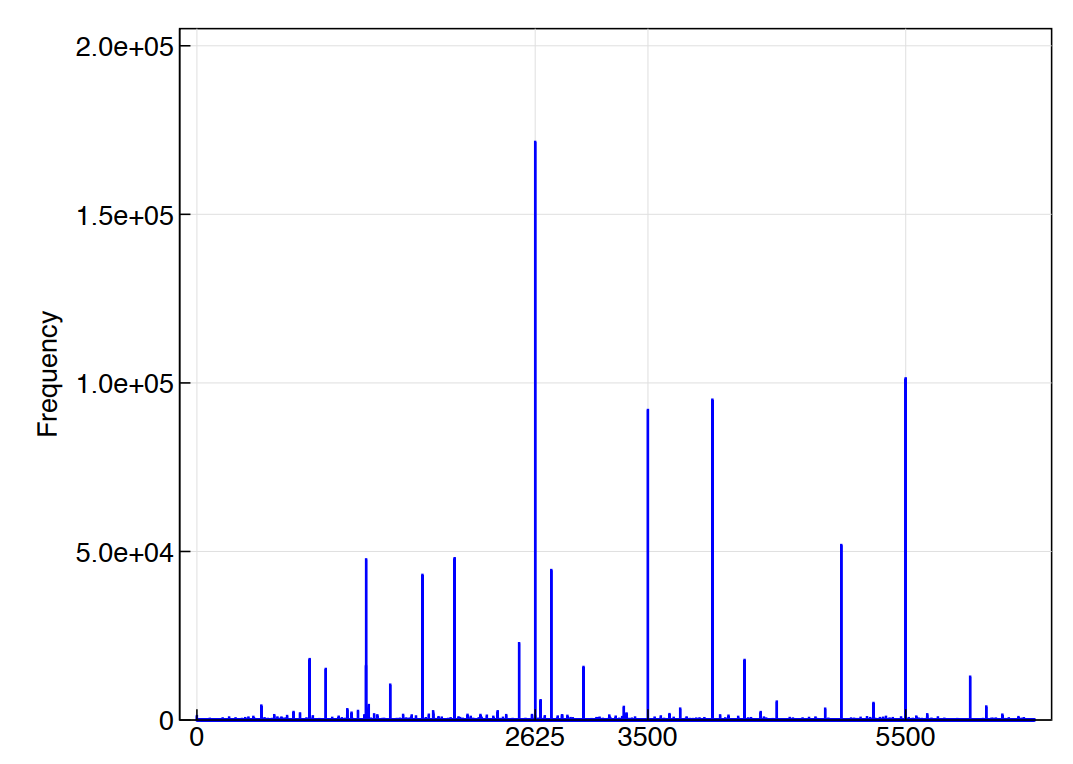
\includegraphics[width = \linewidth]{Lucca6a.png}
		\end{subfigure} 
	\begin{subfigure}{0.49\textwidth}
		\centering
		\caption{Student Loan Frequencies 2007-2008}
		\label{luc07}
		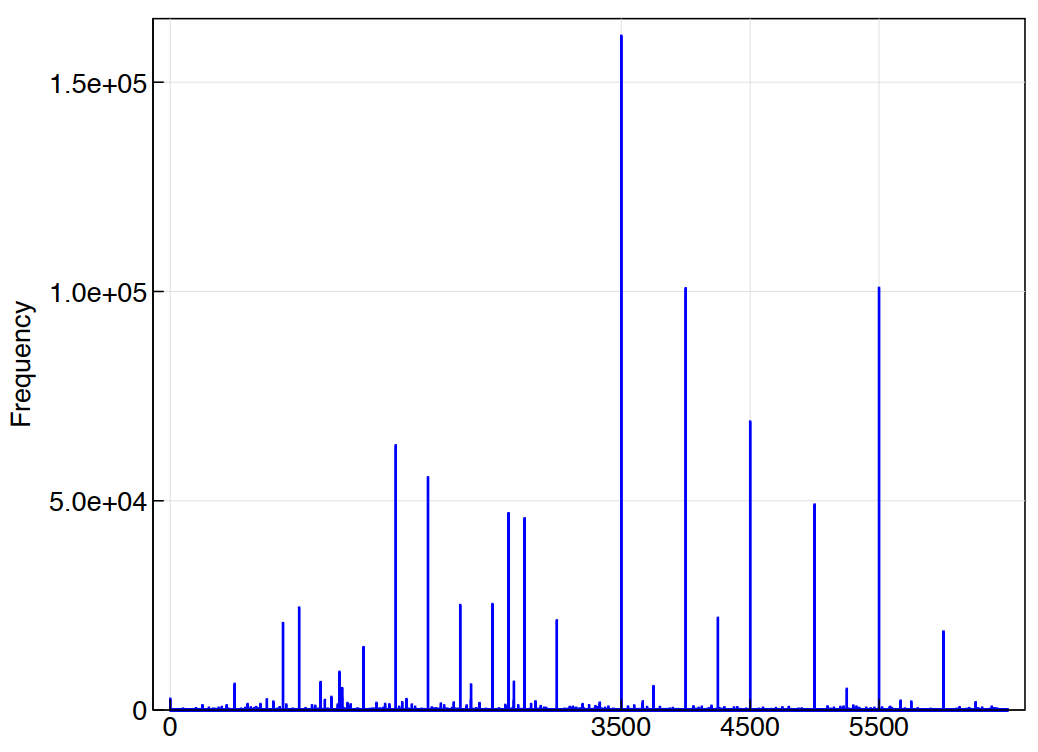
\includegraphics[width = \linewidth]{Lucca6b.png}
		\end{subfigure}
	\end{figure}
	
	\section{Data}
	
	For my paper I use data from the National Longitudinal Survey of Youth '79 Children and Young Adults (NLSY79 CYA). A follow-up to the original National Longitudinal Survey of Youth '79, the CYA surveys the original respondents' children semiyearly from birth until the present day. Thus, we have respondents across the entire age spectrum during the implementation of the policy, allowing us to observe time-varying trends in debt acquisition and career choice. 
	
	The benefits of the CYA data over the Princeton data from \textcite{rothstein2011} are several. First, the NLSY is designed to focus on lower income households rather than Anon U's much wealthier sample. Second, the students in this survey attend a much broader range of colleges than those in the Rothstein data set. As the students who are accepted into prestigious universities such as Anon U are by definition selected, they \emph{cannot} be representative of the general American college-bound population. Third, the CYA surveys students both about their finances and about their career aspirations at each step of the process. Thus, not only can I track student outcomes after graduation, I am able to plot students' intentions over time, tracking variables such as intended major during their time at school. This provides a more interesting, nuanced panel as we can see how students' intentions evolve as their access to credit changes. Finally, with data from several different colleges, we can examine how college traits interact with student debt and career outcomes. 
	
	One drawback of the CYA data set is that, as a survey, many of the figures are less precise than those in other sets. For example, when asked about their level of debt, the vast majority of responses are rounded numbers. While useful for qualitative analysis, this makes it difficult to assess data granularly as done by \textcite{lucca2018} in figure \ref{luc}. Fortunately, because they have a nationally representative dataset, there is no reason to believe their results would differ with our sample. Indeed, as our sample is of lower income relative to the general population, I would argue that subjects are bound more strongly by the policy as for many students federal loans may be their only option for college financing.
	
	Because of the connection between the CYA and original NLSY79, we can import very rich background information for each of our participants. Specifically, for each student we can identify parental income for the year in question among other background traits inherited from parents.
	
	\section{Model}
	
	Our data set is a balanced panel of students surveyed every other year over the years 2000-2010. We conduct a two-stage least squares regression, using exposure to the increased student loan caps as an instrument for total student debt. Note, however, that debt is inherently censored below--students can only have positive values of debt, and those who would receive ``negative'' values are instead observed as 0. Due to this idiosyncrasy, I approach my first stage regression with two strategies.
	
	First, I attempt to use a Tobit model to forecast values for debt. Thus, I would like my first stage model to be $$\ln(debt)_{it} = \delta_0 + \delta_1 treatment_{it} + \delta_2 year_t + \vec{\gamma}^T \vec{\mbox{demographics}}_i + \mu_{it}$$ However, projected values from the Tobit using this model would fail, as errors are only guaranteed to be uncorrelated with fitted values under Ordinary Least Squares. Therefore I use a method suggested by \textcite{angrist2009} whereby the fitted Tobit values are used as an instrument for debt themselves. Thus, we calculate a pre-first stage such that $$\ln(\widehat{debt}')_{it} = \alpha_0 + \alpha_1 \widehat{debt}_{it} + \alpha_2 year_t + \vec{\upsilon}^T \vec{\mbox{demographics}}_i + \mu_{it}$$ These projected values are then used as the values for debt in the second stage. 
	
	[JUSTIFY USE OF CONTROLS]
	
	An alternative specification is that outlined in [PAPER HANDLING WITH DUMMY]. Here, we run our first stage only on students who \emph{have} debt. 
	
	%our first stage equation for students who have debt $> 0$ is $$\ln(\mbox{debt})_{it} = \delta_0 + \delta_1 \mbox{year}_t + \delta_2 \mbox{year $\times$ cohort} + \vec{\gamma}^T \vec{\mbox{demographics}}_i + \mu_{it}$$ In this regression, demographics include traits such as sex, race, parental income, and region of the country where the student lives. 
	
	Using these estimates, we can then produce a second stage regression estimating a variety of career outcomes. For example, we estimate the probability of graduationg with various majors for each student. 
	
	In this example, the model would be $$\mathbb{P}(\mbox{major}_i) = \beta_0 + \beta_1 \widehat{\ln(\mbox{debt})}_{it} + \beta_2 \mbox{hasDebt}_{it} \times \widehat{\ln(\mbox{debt})}_{it} + \vec{\xi}^T \vec{\mbox{demographics}}_i + \epsilon_{it}$$ Note we must have a dummy for whether a student has debt interacted with debt itself due to the bottom censorship of the variable. 
	
	[ALSO CAN ADD EXPECTED EARNINGS ON LEFT SIDE ONCE I ADD THAT DATA]
	
	\section{Results}
	
	\blindtext
	
	\section{Discussion}
	
	\blindtext
	
	\section{Conclusion}
	
	\blindtext

	\printbibliography
	
\end{document}